\section{Final Specifications and Requirements}

To implement the proposed system, the following technical and methodological requirements are outlined:

\begin{itemize}
    \item \textbf{Hardware Requirements:} GPU-enabled computing resources are essential for training and distilling LLMs. Most experiments will be conducted using platforms such as Google Colab, Kaggle Kernels, or institutional GPU servers.
    
    \item \textbf{Software Requirements:}
    \begin{itemize}
        \item Python (≥3.8), PyTorch, HuggingFace Transformers, FAISS for dense retrieval.
        \item Dataset handling using Pandas and preprocessing with SpaCy or NLTK.
        \item Evaluation using standard NLP metrics (BLEU, ROUGE, F1, Accuracy).
    \end{itemize}

    \item \textbf{Data Requirements:} Digitized legal documents in English and Bangla from publicly available sources such as:
    \begin{itemize}
        \item The Bangladesh Laws website.
        \item Judgments from the Supreme Court archive.
        \item Legal aid materials and translated summaries.
    \end{itemize}

    \item \textbf{Deployment Requirements:} The final model will be converted to ONNX or TensorFlow Lite format for mobile deployment. A lightweight interface will be developed using Flutter or React Native, ensuring offline functionality and a minimal memory footprint.
\end{itemize}



\section{Societal Impact}


The proposed system aims to bridge the digital and legal divide by enabling accessible, offline legal assistance for the people of Bangladesh. By leveraging AI on mobile platforms, the project could enhance legal literacy, reduce dependency on costly legal consultations, and empower individuals to make informed legal decisions. Potential impacts include improved access to justice, greater civic awareness, and a model for similar low-resource contexts globally.




\section{Ethical Issues}
The project must ensure that legal advice generated by the system is clearly marked as non-professional and indicative only, to avoid misuse. Bias mitigation, transparency, and fairness in both training data and model behavior are critical. Data privacy and compliance with local legal data usage policies will be strictly maintained.

\section{Standards - if applicable}

While no specific international technical standards are directly mandated for this project, best practices from the fields of Responsible AI, such as those outlined by IEEE and ISO/IEC for trustworthy AI systems, will be adhered to. These include principles of fairness, accountability, transparency, and privacy.

\section{Project Management Plan}
Prepare a project management plan including schedule, budget, and resource management.

\subsection{Breakdown of Pre-Thesis 1}

Our pre-thesis workflow has been broken down into several steps:

\begin{itemize}
    \item Initially, our team aligned their research interests to find a common ground and select a research field to work on.
    \item We studied related research papers to gain a deeper understanding and background knowledge on the selected domain.
    \item A literature review was written based on the most relevant research works.
    \item After gaining sufficient domain knowledge, we compiled our work according to the university-provided template.
    \item We checked for plagiarism and rewrote the necessary segments to ensure the overall similarity index remained below 15\%.
    \item Once all issues were addressed, we submitted the final version of our Pre-Thesis 1 paper.
\end{itemize}

\begin{figure}
    \centering
    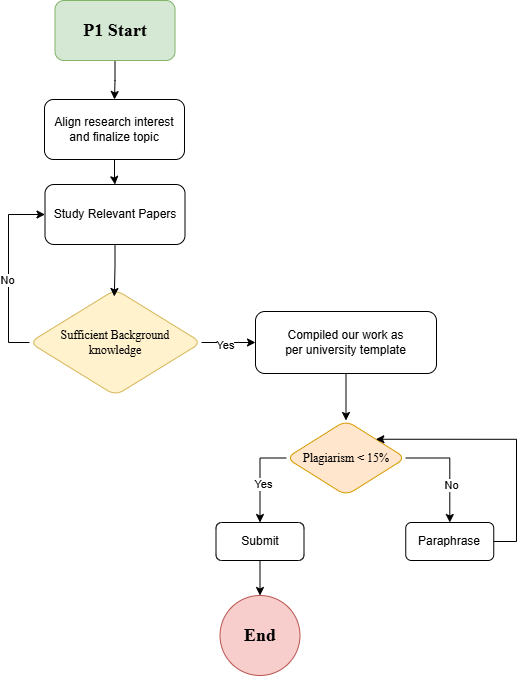
\includegraphics[width=0.6\linewidth]{images/p1_breakdown_1.drawio.png}
    \caption{Workflow of Pre-thesis 01}
    \label{fig:Workflow of Pre-thesis 01}
\end{figure}



\subsection{Tentative Breakdown of Pre-Thesis 2}

Our initial research plan involves proposing a lightweight and domain-specific Retrieval-Augmented Generation (RAG) framework optimized for the legal domain in Bangladesh. The following tasks are planned for Pre-Thesis 2:

\begin{itemize}
    \item Collect and preprocess legal datasets (e.g., laws, verdicts, regulations) relevant to the Bangladeshi legal system.
    \item Implement a basic legal document retriever using both traditional and neural retrieval methods.
    \item Fine-tune or adapt a medium or small-sized LLM to the legal domain and evaluate it using standard NLP metrics such as Accuracy, F1-score, BLEU, and ROUGE.
    \item Integrate the retriever and generator to build an initial RAG pipeline.
    \item Conduct qualitative and quantitative evaluations to identify limitations.
    \item Generate a baseline report focusing on generation quality, latency, and legal accuracy.
\end{itemize}

\begin{figure}[H]
    \centering
    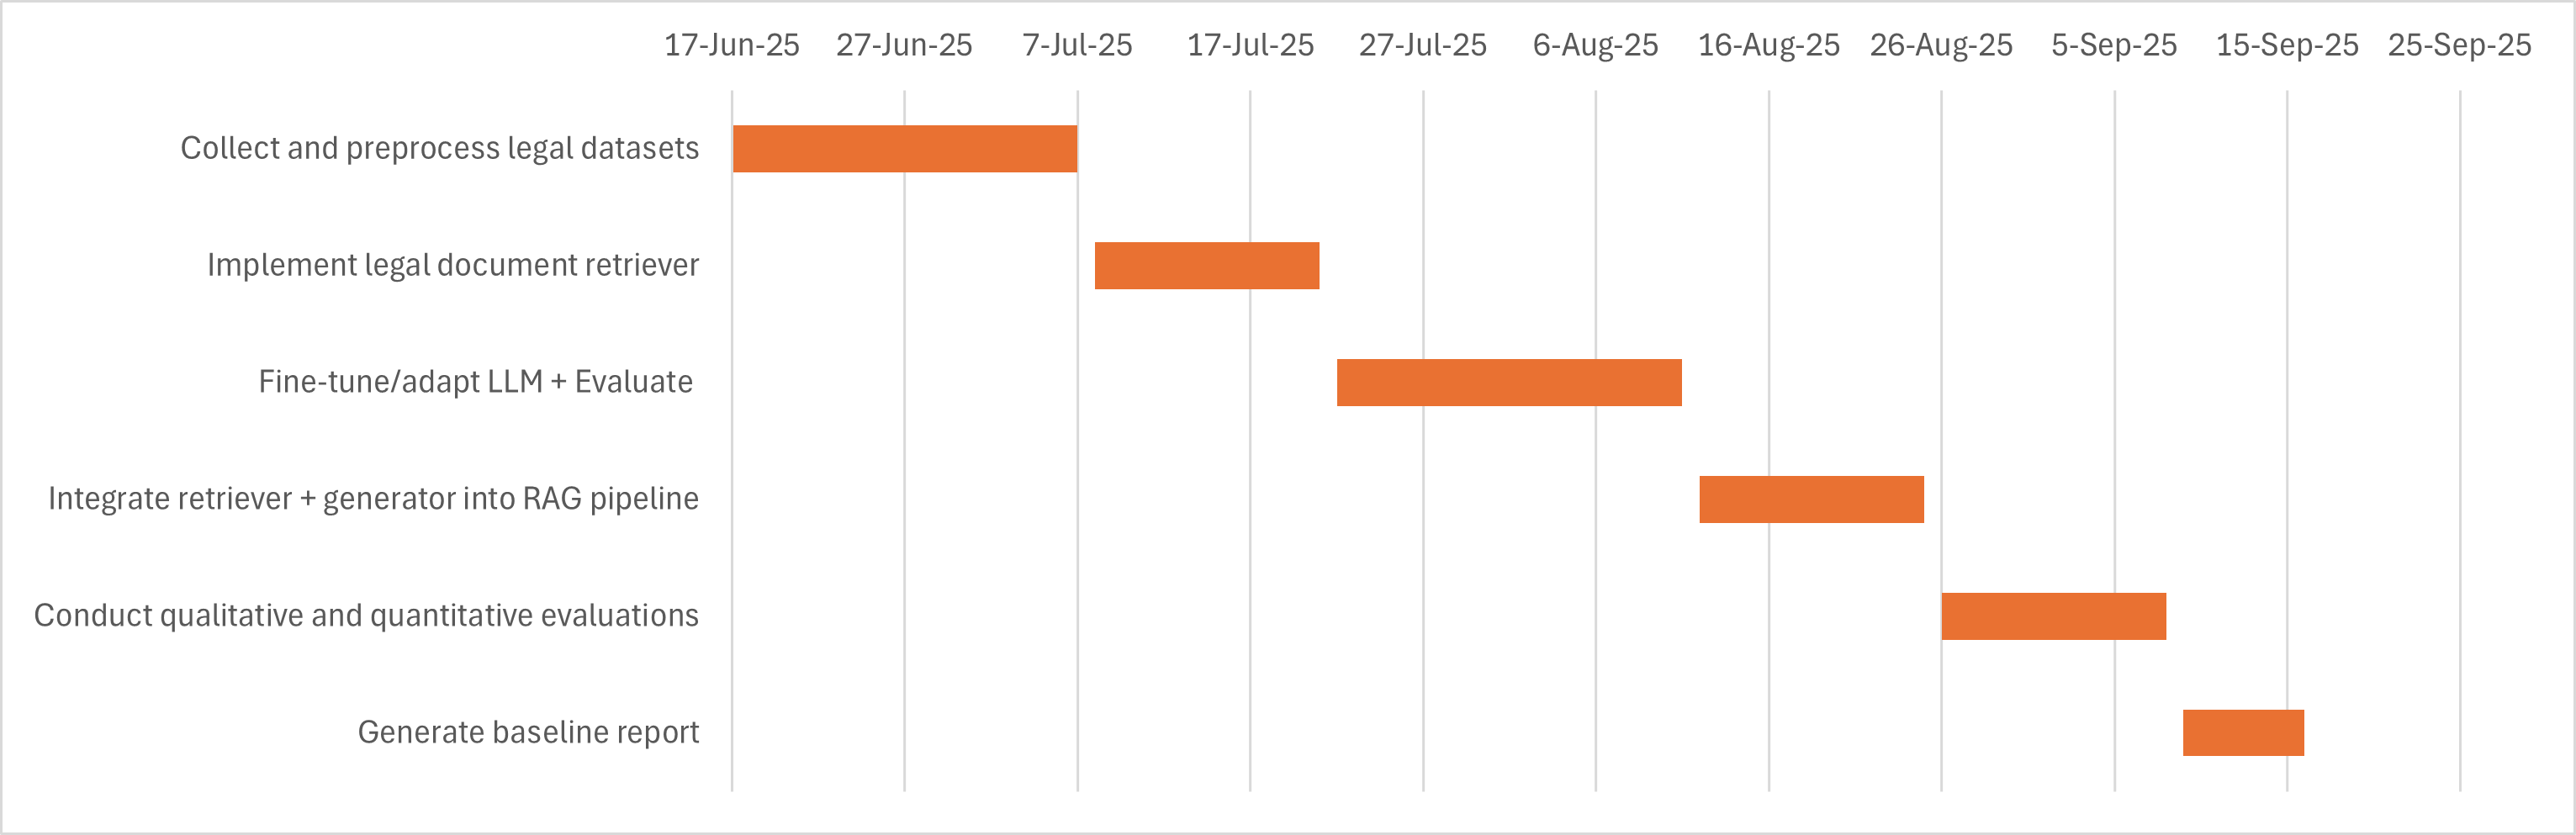
\includegraphics[width=1.0\linewidth]{images/Gantt Chart.png}
    \caption{Gantt chart illustrating the project workflow}
    \label{fig:Gantt chart illustrating the project workflow}
\end{figure}
\subsection{Thesis Defense}

For the final defense, we plan to finalize the distilled and optimized RAG pipeline for legal information access. The tasks to be completed include:

\begin{itemize}
    \item Finalize and evaluate the optimized legal RAG framework.
    \item Prepare a detailed technical report and comprehensive documentation.
    \item Analyze the strengths, weaknesses, and real-world applicability of the system.
    \item Write and submit a research paper summarizing methodology, experiments, and results.
    \item Open-source the project with clean documentation to encourage community involvement and further development.
    \item Identify and submit the work to a suitable peer-reviewed journal or conference in the fields of AI, NLP, or LegalTech.
\end{itemize}


\section{Economic Analysis}


The economic viability of the proposed system involves both development and potential deployment costs. As the system is designed to be resource-efficient and accessible, cost-effective development strategies have been prioritized.

\begin{itemize}
    \item \textbf{GPU Resources:} The majority of model training and experimentation will be conducted using:
    \begin{itemize}
        \item Google Colab Pro: Approx.\ \$10/month for access to T4 or P100 GPUs.
        \item Google Colab Pro+: Approx.\ \$50/month for A100 GPUs and extended runtimes.
        \item Kaggle Kernels: Free GPU access for light preprocessing and testing.
    \end{itemize}
    
    \item \textbf{Software Tools:} All core libraries and frameworks (e.g., PyTorch, Transformers, FAISS, NLTK, SpaCy) are open-source, thus incurring no direct licensing cost.

    \item \textbf{Data Acquisition:} All legal documents are sourced from publicly available government or institutional portals, minimizing data procurement costs.

    \item \textbf{Deployment Costs:} 
    \begin{itemize}
        \item Edge deployment using ONNX or TensorFlow Lite involves no licensing fee.
        \item Mobile front-end development with Flutter or React Native is open-source and free to use.
    \end{itemize}

    \item \textbf{Maintenance and Scalability:} Future maintenance and updates may require continued access to GPU resources and developer time. Community-based open-source collaboration could help reduce long-term costs.

\end{itemize}

Overall, the proposed solution is designed to be cost-effective, with major recurring expenses limited to training compute time on cloud GPU platforms during development phases.
